% !TeX root = skript.tex
Eine elementare Aufgabe in Network Science ist es die Wichtigkeit von Knoten zu bewerten --- man spricht auch \aside{Zentralität: Wichtigkeit eines Knotens} von der \emph{Zentralität} der Knoten.
Die Anzahl der Nachbarn (Grad, engl. degree) ist eine sehr einfache Metrik mit eingänglicher Intuition:
wenn ein Knoten überdurchschnittlich viele Nachbarn hat, dann steht die Vermutung im Raum, dass diesem Knoten auch eine überdurchschnittlich wichtige Funktion im Netzwerk zu kommt.
Daher wollen wir die Verteilung von Graden in Graphen in diesen Kapitel genauer betrachten.

Zur Wiederholung:
In einem ungerichteten Graphen~$G=(V,E)$ beschreibt
\begin{align}
    \deg(u) = \card{\twoset{e}{e \in E\text{, s.d. } u \in e}}
\end{align}
die Anzahl der Nachbarn von Knoten~$u$.
Die \aside{Grad\underline{sequenz}} Gradsequenz~$\degseq_G$ (falls $G$ klar ist auch nur $\degseq$) von $G=(V,E)$ mit $V=\set{v_1, \ldots, v_n}$ ist dann einfach die Auflistung aller Grade im Graphen
\begin{align}
    \degseq_G = (\deg(v_1), \deg(v_2), \ldots, \deg(v_n)).
\end{align}
Beobachte, dass für jede $\degseq_G$ von $G=(V,E)$ gilt:
\begin{align}
    \sum_{v \in V} \deg(v) = 2 \card{E}
\end{align}


\section{Knotengrade in $\Gnp$}
\begin{figure}
    \begin{center}
        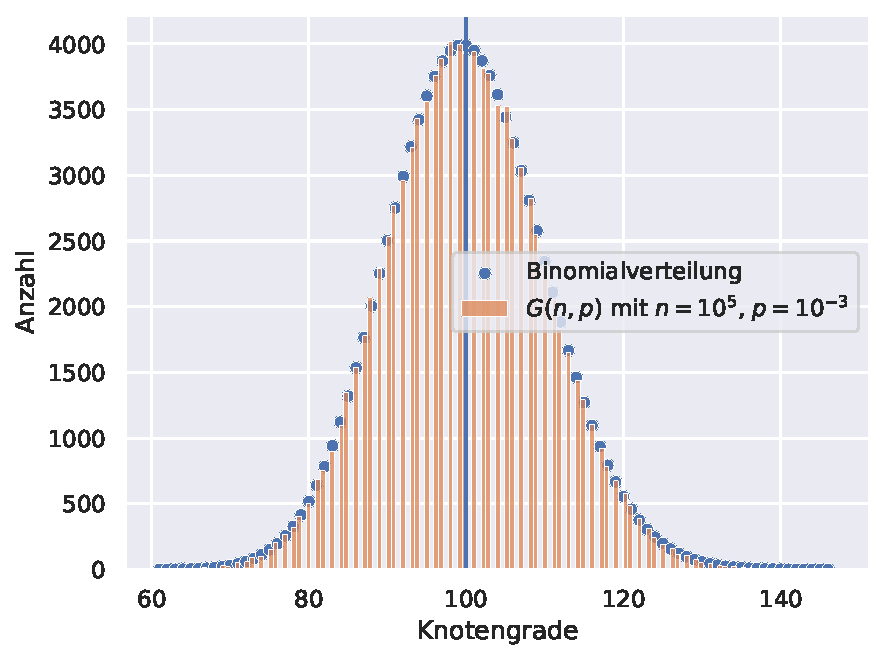
\includegraphics[width=0.6\textwidth]{data/gnp_degrees.pdf}
    \end{center}
    \caption{
        Histogram der Gradsequenz~$\degseq_G$ eines Graphen~$G \sim \Gnp$.
        Die vertikale Linie zeigt den Durchschnittsgrad $\bar k$,
        die Punkte die Vorhersage mittels Binomialverteilung.
    }
    \label{fig:histogram_grade_gnp}
\end{figure}

Die Gradsequenz~$\degseq_G$ ist ein konkreter \qq{Messwert} für einen Graph~$G$.
Für die meisten Graphen mit vielen Knoten können wir --vereinfachend-- davon ausgehen, dass die einzelnen Grade unabhängig aus einer Wahrscheinlichkeitsverteilung gezogen wurden.
Wir \aside{Grad\underline{verteilung}} nennen diese Wahrscheinlichkeitsverteilung dann die \emph{Gradverteilung}.
Das ist besonders sinnvoll, wenn $G$ selbst aus einem Zufallsgraph stammt.
Dann versuchen wir die Gradverteilung auf das durch den Zufallsgraphen definierte Ensemble auszuweiten.
Im folgenden betrachten wir etwa die Gradverteilung von $\Gnp$ Graphen.

Aus \cref{subsec:anzahl_kanten_in_gnp} wissen wir bereits, dass die Kantenanzahl eines $\Gnp$ Graphen binomial verteilt ist.
Die Analyse für Grade läuft analog, allerdings nicht für $\binom n 2$ Einträge der Adjazenzmatrix, sondern nur für $n-1$ (da Eigenschleifen verboten sind: $-1$).
Der Grad~$\deg(u)$ eines Knotens~$u$ ist also ebenfalls binomial verteilt:
\begin{align}
    \prob{\deg(u) = k} =
    \underbrace{\binom{n-1}{k}}_\text{\begin{minipage}{9em}\centering Anzahl an möglichen\\[-0.5em] Nachbarschaften\end{minipage}}
    \ \cdot \
    \underbrace{p^k}_\text{Existenz der $k$ Kanten}
    \ \cdot \
    \underbrace{(1-p)^{n-1-k}}_\text{\begin{minipage}{10em}\centering Abwesenheit der \\[-0.5em] restlichen Kanten\end{minipage}}
    \label{eq:gradverteilung_gnp}
\end{align}
Daher gilt also $\expv{\deg(u)} = (n-1)p$.

Wie in \cref{fig:histogram_grade_gnp} dargestellt, approximiert eine konkrete Gradsequenz~$\degseq_G$ die Gradverteilung schon sehr gut.
Der Erwartungswert sollte daher gegen den Durchschnittsgrad $\bar d = 2m / n$ konvergieren, d.h. $\expv{\deg(u)} \approx \bar d$.
Dann gilt also:
\begin{align}
    \bar d \approx \expv{\deg(u)} & = (n-1)p \\
    p \approx \frac{\bar d}{n-1} \label{eq:gnp_p_von_avg_deg}
\end{align}

Für tiefere analytische Untersuchen ist die Binomialverteilung ein bisschen unhandlich.
Wir wollen daher eine Approximation (siehe \cite{barabasi2014network}) für dünne Netzwerke finden.
Aus $m = \Oh{n \log n}$ folgt direkt $\bar d = \Oh{\log n}$.
Somit ist also $\bar d \ll n$ eine gute Annahme für dünne Graphen.

\medskip

Betrachten wir also zunächst den Binomialkoeffizienten in \cref{eq:gradverteilung_gnp}:
\begin{align}
    \binom{n-1}{k}
     & = \frac{1}{k!} \cdot \frac{(n-1)!}{(n-1-k)!}                                                              \\
     & = \frac{1}{k!} \cdot \left[ (n-1) \cdot (n-1-1) \cdot (n-1-2) \cdot \ldots \cdot (n-1-(k - 1))    \right] \\
     & \approx \frac{1}{k!} \left[ n- 1 \right]^k
\end{align}

Im letzten Schritt nutzten wir aus, dass $k \ll n$ und somit $n-1 \approx n-k$.
Die Wahrscheinlichkeit, in \cref{eq:gradverteilung_gnp}, dass $n-1-k$ Nachbarn \emph{nicht} existieren, können wir wie folgt auffassen:
\begin{align}
    (1 - p)^{n-1-k} & = \exp\left[ \ln\left((1 - p)^{n-1-k}  \right) \right]
\end{align}

\noindent
Konzentrieren wir uns nun zunächst auf den Logarithmus:
\begin{align}
    \ln\left((1 - p)^{n-1-k}  \right)  =
    (n-1-k) \ln (1 - p)
    \approx - (n-1-k) p
\end{align}

\noindent
Im letzten Schritt nutzen wir die Abschätzung $\ln(1+x) \approx x$, welche für kleine $x \ll 1$ aus der Taylorreihe von $\ln(1+x) = x - \Oh{x^2}$ resultiert.
Nun können wir \cref{eq:gnp_p_von_avg_deg} nutzen, um $p$ zu substituieren:
\begin{align}
    - (n-1-k) p \approx - (n-1-k) \frac{\bar d}{n-1} \approx - \bar d
\end{align}

\noindent
Somit folgt letztendlich:
\begin{align}
    (1 - p)^{n-1-k} = \exp\left[ \ln\left((1 - p)^{n-1-k}  \right) \right] \approx \exp(-\bar d)
\end{align}

\noindent
Damit haben wir nun alle Bausteine, um die Binomialverteilung zu approximieren:
\begin{align}
    \prob{\deg(u) = k}
     & = \textcolor{red}{\binom{n-1}{k}} \cdot p^k \cdot \textcolor{blue}{(1-p)^{n-1-k}}                       \\
     & \approx \textcolor{red}{\frac{1}{k!} \left[ n- 1 \right]^k} p^k \textcolor{blue}{\exp(-\bar d)}         \\
     & \stackrel{(\ref{eq:gnp_p_von_avg_deg})}{\approx}
    \textcolor{red}{\frac{1}{k!} \left[ n- 1 \right]^k} [\frac{\bar d}{n-1}]^k \textcolor{blue}{\exp(-\bar d)} \\
     & = \frac{\bar d^k}{k!} \exp(-\bar d)
\end{align}

\noindent
Beim letzten Ausdruck handelt es sich um die Poissonverteilung:

\begin{definition}
    Für \aside{Poissonverteilung} $\lambda > 0$ ist die ganzzahlige und nicht-negative Zufallsvariable $X$ \emph{poisson-verteilt}, falls
    \begin{align}
        \prob{X = k} = \frac{\lambda ^k}{k!} \exp(-\lambda)
    \end{align}

    Dann gilt, dass der Erwartungswert $\expv{X} = \lambda$ und die Varianz $\var(X) = \lambda$ identisch sind.
\end{definition}

\begin{figure}
    \begin{center}
        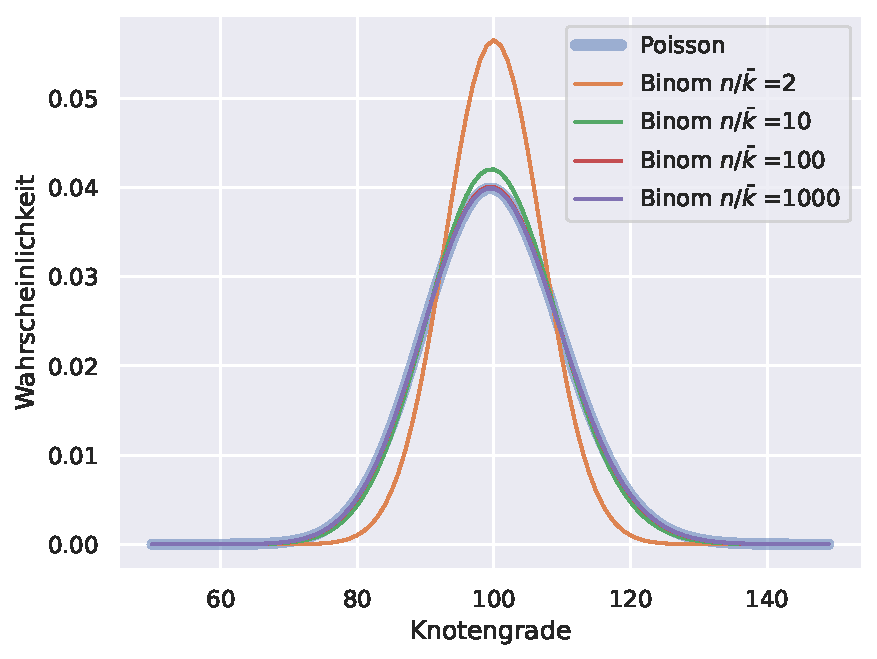
\includegraphics[width=0.5\textwidth]{data/binom_vs_poisson.pdf}
    \end{center}
    \caption{
        Vergleich von Binomialverteilung und Poissonverteilung für fixierten Durchschnittsgrad $\bar k = 100$.
        Je größer $n$, desto eher ist die Approximationsvoraussetzung $\bar k \ll n$ erfüllt, und desto mehr sind Binomialverteilung und Poissonverteilung deckungsgleich.
    }
    \label{fig:binom_vs_poisson}
\end{figure}

\bigskip

Aus dieser Approximation mittels Poissonverteilung ergibt sich eine interessante Einsicht.
Während \aside{Für $\bar k \ll n$ ist die Gradverteilung nur von $\bar k$ abhängig} die Binomialverteilung von der Knotenanzahl~$n$ und Kantenwahrscheinlichkeit~$p$ abhängt, hat die Poissonverteilung nur den Parameter~$\lambda = p / (n-1) \approx \bar k$.
Die Interpretation hiervon ist, dass für $\bar k \ll n$ die Gradverteilung nur vom Durchschnittsgrad~$\bar k$, nicht aber von der Knotenanzahl im Graphen abhängen sollte.
\Cref{fig:binom_vs_poisson} untermauert diese Interpretation: die Binomialverteilungen der zwei größten Netze sind mit dem bloßen Auge nicht mehr von der Poissonverteilung unterscheidbar.

Diese Einsicht können wir uns wie folgt erklären:
Die Poissonverteilung beschreibt die Anzahl von Ereignissen, die innerhalb eines fixierten Intervalls auftreten, wenn die mittlere Rate konstant ist.
In diesem Bild ist jede Zeile der Adjazenzmatrix solch ein Intervall und die mittlere Rate entspricht der durchschnittlichen Anzahl an Einsen pro Zeile --- also dem Durchschnittsgrad~$\bar d$.

Beachte auch, dass die Varianz der Poissonverteilung mit $\var(X) = \bar d$ größer ist als die Varianz der Binomialverteilung $\var(X) = n p(1 - p) \approx \bar d (1 - \bar d / n )$, wobei der geklammerte Faktor kleiner als $1$ ist.

\section{Powerlaw Gradverteilung}
\begin{figure}
    \begin{center}
        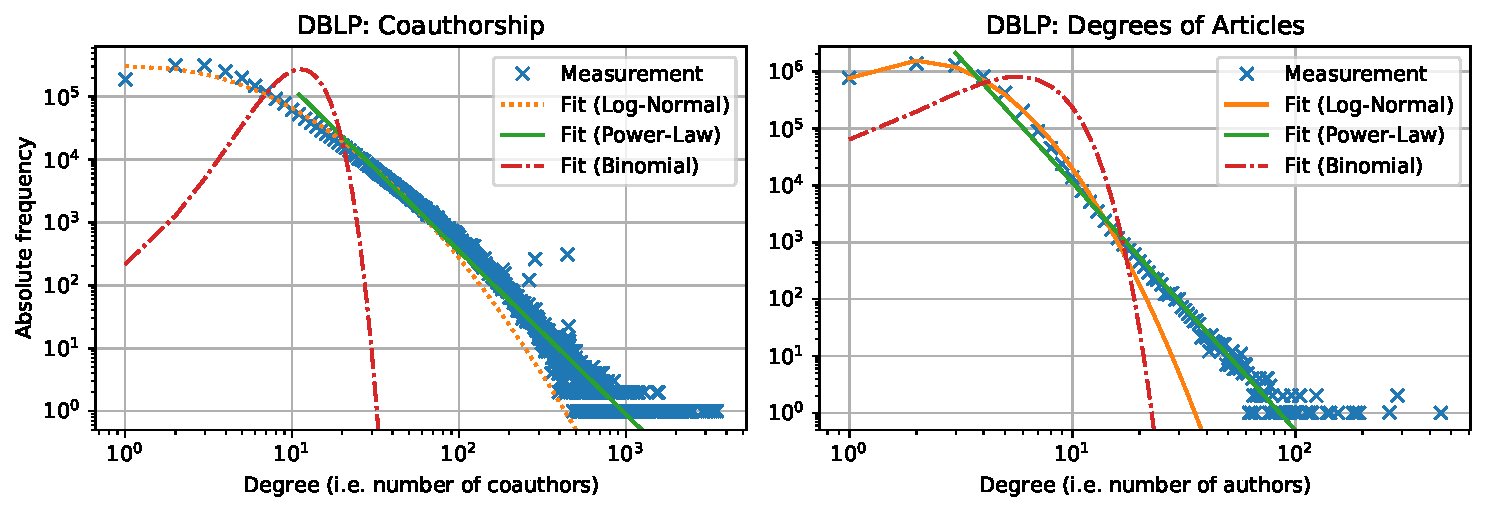
\includegraphics[width=\textwidth]{data/dblp_degree_distribution.pdf}
    \end{center}
    \caption{Gradverteilung von zwei beobachteten Netzwerken~\cite{Penschuck_2020} verglichen mit drei analytischen Verteilungen.}
    \label{fig:grade_in_dblp}
\end{figure}

In \cref{fig:grade_in_dblp} stellen wir die Gradverteilung, genauer das Histogram der Gradsequenz, von zwei beobachteten Netzwerken dar.
Die genaue Herkunft der Graphen ist hier nicht wichtig; viele beobachte komplexe Netzwerke zeigen einen qualitativ ähnlichen Verlauf.
Was sofort auffällt, ist, dass die rot dargestellte Binomialverteilung keine satisfaktionsfähige Übereinstimmung mit der beobachteten Verteilung zeigt:

\begin{itemize}
    \item Die Binomialverteilung sagt vorher, dass die meisten Knoten grob den Durchschnittsgrad haben müssten.
          Zu beiden Richtungen ---sprich für kleinere und größere Grade--- sollte es deutlich weniger Knoten geben.

    \item Der maximale Grad ($\approx 30$ im linken Schaubild) sollte in etwa dieselbe Größenordnung haben, wie der Durchschnittsgrad ($\approx 10$).
\end{itemize}

\noindent
Das beobachtete Netzwerk hat jedoch ein signifikant anderes Verhalten:
\begin{itemize}
    \item Die meisten Knoten haben sehr geringen Grad --- deutlich geringer als der Durchschnittsgrad.
    \item Der maximal Grad ($\approx 4000$) ist viel höher als der Durchschnittsgrad ($\approx 10$).
          Offensichtlich \qq{ziehen} diese wenigen Knoten den Durchschnittsgrad also maßgeblich nach oben.
          Es sollte daher auch nicht überraschend, dass diese sog. Hubs viele Eigenschaften des Netzwerks prägen.
\end{itemize}



